\documentclass[a4paper,14pt,oneside,openany]{memoir}
\usepackage[utf8]{inputenc}

%%% Задаем поля, отступы и межстрочный интервал %%%

\usepackage[left=30mm, right=15mm, top=20mm, bottom=20mm]{geometry} % Пакет geometry с аргументами для определения полей
\pagestyle{plain} % Убираем стандарные для данного класса верхние колонтитулы с заголовком текущей главы, оставляем только номер страницы снизу по центру
\parindent=1.25cm % Абзацный отступ 1.25 см, приблизительно равно пяти знакам, как по ГОСТ
\usepackage{indentfirst} % Добавляем отступ к первому абзацу
%\linespread{1.3} % Межстрочный интервал (наиболее близко к вордовскому полуторному) - тут вместо этого используется команда OnehalfSpacing*

%%% Задаем языковые параметры и шрифт %%%

\usepackage[english, russian]{babel}                % Настройки для русского языка как основного в тексте
\babelfont[russian]{rm}{Times New Roman}                     % TMR в качестве базового roman-щрифта



%%% Задаем стиль заголовков и подзаголовков в тексте %%%

\setsecnumdepth{subsection} % Номера разделов считать до третьего уровня включительно, т.е. нумеруются только главы, секции, подсекции
\renewcommand*{\chapterheadstart}{} % Переопределяем команду, задающую отступ над заголовком, чтобы отступа не было
\renewcommand*{\printchaptername}{} % Переопределяем команду, печатающую слово "Глава", чтобы оно не печалось
%\renewcommand*{\printchapternum}{} % То же самое для номера главы - тут не надо, номер главы оставляем
\renewcommand*{\chapnumfont}{\normalfont\bfseries} % Меняем стиль шрифта для номера главы: нормальный размер, полужирный
\renewcommand*{\afterchapternum}{\hspace{1em}} % Меняем разделитель между номером главы и названием
\renewcommand*{\printchaptertitle}{\normalfont\bfseries\centering\MakeUppercase} % Меняем стиль написания для заголовка главы: нормальный размер, полужирный, центрированный, заглавными буквами
\setbeforesecskip{20pt} % Задаем отступ перед заголовком секции
\setaftersecskip{20pt} % Ставим такой же отступ после заголовка секции
\setsecheadstyle{\raggedright\normalfont\bfseries} % Меняем стиль написания для заголовка секции: выравнивание по правому краю без переносов, нормальный размер, полужирный
\setbeforesubsecskip{20pt} % Задаем отступ перед заголовком подсекции
\setaftersubsecskip{20pt} % Ставим такой же отступ после заголовка подсекции
\setsubsecheadstyle{\raggedright\normalfont\bfseries}  % Меняем стиль написания для заголовка подсекции: выравнивание по правому краю без переносов, нормальный размер, полужирный

%%% Задаем параметры оглавления %%%

\addto\captionsrussian{\renewcommand\contentsname{Содержание}} % Меняем слово "Оглавление" на "Содержание"
\setrmarg{2.55em plus1fil} % Запрещаем переносы слов в оглавлении
%\setlength{\cftbeforechapterskip}{0pt} % Эта команда убирает интервал между заголовками глав - тут не надо, так красивее смотрится
\renewcommand{\aftertoctitle}{\afterchaptertitle \vspace{-\cftbeforechapterskip}} % Делаем отступ между словом "Содержание" и первой строкой таким же, как у заголовков глав
%\renewcommand*{\chapternumberline}[1]{} % Делаем так, чтобы номер главы не печатался - тут не надо
\renewcommand*{\cftchapternumwidth}{1.5em} % Ставим подходящий по размеру разделитель между номером главы и самим заголовком
\renewcommand*{\cftchapterfont}{\normalfont\MakeUppercase} % Названия глав обычным шрифтом заглавными буквами
\renewcommand*{\cftchapterpagefont}{\normalfont} % Номера страниц обычным шрифтом
\renewcommand*{\cftchapterdotsep}{\cftdotsep} % Делаем точки до номера страницы после названий глав
\renewcommand*{\cftdotsep}{1} % Задаем расстояние между точками
\renewcommand*{\cftchapterleader}{\cftdotfill{\cftchapterdotsep}} % Делаем точки стандартной формы (по умолчанию они "жирные")
\maxtocdepth{subsection} % В оглавление попадают только разделы первыхтрех уровней: главы, секции и подсекции

%%% Выравнивание и переносы %%%

%% http://tex.stackexchange.com/questions/241343/what-is-the-meaning-of-fussy-sloppy-emergencystretch-tolerance-hbadness
%% http://www.latex-community.org/forum/viewtopic.php?p=70342#p70342
\tolerance 1414
\hbadness 1414
\emergencystretch 1.5em                             % В случае проблем регулировать в первую очередь
\hfuzz 0.3pt
\vfuzz \hfuzz
%\dbottom
%\sloppy                                            % Избавляемся от переполнений
\clubpenalty=10000                                  % Запрещаем разрыв страницы после первой строки абзаца
\widowpenalty=10000                                 % Запрещаем разрыв страницы после последней строки абзаца
\brokenpenalty=4991                                 % Ограничение на разрыв страницы, если строка заканчивается переносом

%%% Объясняем компилятору, какие буквы русского алфавита можно использовать в перечислениях (подрисунках и нумерованных списках) %%%
%%% По ГОСТ нельзя использовать буквы ё, з, й, о, ч, ь, ы, ъ %%%
%%% Здесь также переопределены заглавные буквы, хотя в принципе они в документе не используются %%%

\makeatletter
    \def\russian@Alph#1{\ifcase#1\or
       А\or Б\or В\or Г\or Д\or Е\or Ж\or
       И\or К\or Л\or М\or Н\or
       П\or Р\or С\or Т\or У\or Ф\or Х\or
       Ц\or Ш\or Щ\or Э\or Ю\or Я\else\xpg@ill@value{#1}{russian@Alph}\fi}
    \def\russian@alph#1{\ifcase#1\or
       а\or б\or в\or г\or д\or е\or ж\or
       и\or к\or л\or м\or н\or
       п\or р\or с\or т\or у\or ф\or х\or
       ц\or ш\or щ\or э\or ю\or я\else\xpg@ill@value{#1}{russian@alph}\fi}
\makeatother

%%% Задаем параметры оформления рисунков и таблиц %%%

\usepackage{graphicx, caption, subcaption} % Подгружаем пакеты для работы с графикой и настройки подписей
\graphicspath{{images/}} % Определяем папку с рисунками
\captiondelim{ --- } % Разделителем между номером рисунка/таблицы и текстом в подписи является длинное тире
\setkeys{Gin}{width=\textwidth} % По умолчанию размер всех добавляемых рисунков будет подгоняться под ширину текста
\renewcommand{\thesubfigure}{\asbuk{subfigure}} % Нумерация подрисунков строчными буквами кириллицы
%\setlength{\abovecaptionskip}{0pt} % Отбивка над подписью - тут не меняем
%\setlength{\belowcaptionskip}{0pt} % Отбивка под подписью - тут не меняем
\usepackage[section]{placeins} % Объекты типа float (рисунки/таблицы) не вылезают за границы секциии, в которой они объявлены

%%% Задаем параметры ссылок и гиперссылок %%% 

\usepackage{hyperref}                               % Подгружаем нужный пакет
\hypersetup{
    colorlinks=true,                                % Все ссылки и гиперссылки цветные
    linktoc=all,                                    % В оглавлении ссылки подключатся для всех отображаемых уровней
    linktocpage=true,                               % Ссылка - только номер страницы, а не весь заголовок (так выглядит аккуратнее)
    linkcolor=red,                                  % Цвет ссылок и гиперссылок - красный
    citecolor=red                                   % Цвет цитировний - красный
}

%%% Настраиваем отображение списков %%%

\usepackage{enumitem}                               % Подгружаем пакет для гибкой настройки списков
\renewcommand*{\labelitemi}{\normalfont{--}}        % В ненумерованных списках для пунктов используем короткое тире
\makeatletter
    \AddEnumerateCounter{\asbuk}{\russian@alph}     % Объясняем пакету enumitem, как использовать asbuk
\makeatother
\renewcommand{\labelenumii}{\asbuk{enumii})}        % Кириллица для второго уровня нумерации
\renewcommand{\labelenumiii}{\arabic{enumiii})}     % Арабские цифры для третьего уровня нумерации
\setlist{noitemsep, leftmargin=*}                   % Убираем интервалы между пунками одного уровня в списке
\setlist[1]{labelindent=\parindent}                 % Отступ у пунктов списка равен абзацному отступу
\setlist[2]{leftmargin=\parindent}                  % Плюс еще один такой же отступ для следующего уровня
\setlist[3]{leftmargin=\parindent}                  % И еще один для третьего уровня

%%% Счетчики для нумерации объектов %%%

\counterwithout{figure}{chapter}                    % Сквозная нумерация рисунков по документу
\counterwithout{equation}{chapter}                  % Сквозная нумерация математических выражений по документу
\counterwithout{table}{chapter}                     % Сквозная нумерация таблиц по документу

%%% Реализация библиографии пакетами biblatex и biblatex-gost с использованием движка biber %%%

\usepackage{csquotes} % Пакет для оформления сложных блоков цитирования (biblatex рекомендует его подключать)
\usepackage[%
backend=biber,                                      % Движок
bibencoding=utf8,                                   % Кодировка bib-файла
sorting=none,                                       % Настройка сортировки списка литературы
style=gost-numeric,                                 % Стиль цитирования и библиографии по ГОСТ
language=auto,                                      % Язык для каждой библиографической записи задается отдельно
autolang=other,                                     % Поддержка многоязычной библиографии
sortcites=true,                                     % Если в квадратных скобках несколько ссылок, то отображаться будут отсортированно
movenames=false,                                    % Не перемещать имена, они всегда в начале библиографической записи
maxnames=5,                                         % Максимальное отображаемое число авторов
minnames=3,                                         % До скольки сокращать число авторов, если их больше максимума
doi=false,                                          % Не отображать ссылки на DOI
isbn=false,                                         % Не показывать ISBN, ISSN, ISRN
]{biblatex}[2016/09/17]
\DeclareDelimFormat{bibinitdelim}{}                 % Убираем пробел между инициалами (Иванов И.И. вместо Иванов И. И.)
\addbibresource{bibl.bib}                           % Определяем файл с библиографией

%%% Скрипт, который автоматически подбирает язык (и, следовательно, формат) для каждой библиографической записи %%%
%%% Если в названии работы есть кириллица - меняем значение поля langid на russian %%%
%%% Все оставшиеся пустые места в поле langid заменяем на english %%%

\DeclareSourcemap{
  \maps[datatype=bibtex]{
    \map{
        \step[fieldsource=title, match=\regexp{^\P{Cyrillic}*\p{Cyrillic}.*}, final]
        \step[fieldset=langid, fieldvalue={russian}]
    }
    \map{
        \step[fieldset=langid, fieldvalue={english}]
    }
  }
}

%%% Прочие пакеты для расширения функционала %%%

\usepackage{listings}
\usepackage{xcolor}
\lstdefinelanguage{Kotlin}{
  morekeywords={package, import, class, object, interface, fun, val, var,
                if, else, when, for, while, do, return, break, continue,
                is, in, !in, as, !as, null, this, super, try, catch, finally},
  sensitive=true,
  morecomment=[l]{//},
  morecomment=[s]{/*}{*/},
  morestring=[b]",
  morestring=[s]{"""}{"""},
}

\lstset{
  language=Kotlin,
  inputencoding=utf8,        % поддержка UTF-8
  extendedchars=true,        % разрешить расширенные символы
  basicstyle=\ttfamily\small,
  keywordstyle=\color{orange}\bfseries,
  commentstyle=\color{gray}\itshape,    % теперь русские комментарии будут видны
  stringstyle=\color{purple},
  numbers=left,
  numberstyle=\tiny,
  frame=single,
  breaklines=true,
  showstringspaces=false
}
\usepackage{longtable,ltcaption}                    % Длинные таблицы
\usepackage{multirow,makecell}                      % Улучшенное форматирование таблиц
\usepackage{booktabs}                               % Еще один пакет для красивых таблиц
\usepackage{soulutf8}                               % Поддержка переносоустойчивых подчёркиваний и зачёркиваний
\usepackage{icomma}                                 % Запятая в десятичных дробях
\usepackage{hyphenat}                               % Для красивых переносов
\usepackage{textcomp}                               % Поддержка "сложных" печатных символов типа значков иены, копирайта и т.д.
\usepackage[version=4]{mhchem}                      % Красивые химические уравнения
\usepackage{amsmath}                                % Усовершенствование отображения математических выражений 
\usepackage[T2A]{fontenc}
\usepackage[english,russian]{babel}
\usepackage{geometry}
  \geometry{
    a4paper,
    top=2cm,
    bottom=2cm,
    left=3cm,
    right=1.5cm,
    headheight=1cm,
    headsep=0.5cm,
    footskip=1cm
  }
\usepackage{microtype}       % для лучшей переносимости
\usepackage{indentfirst}     % абзацный отступ в начале раздела
\setlength{\parindent}{1.25cm}
\setlength{\parskip}{0pt}
\sloppy

%%% Вставляем по очереди все содержательные части документа %%%

\begin{document}

\thispagestyle{empty}

\begin{center}
    МИНИСТЕРСТВО ЦИФРОВОГО РАЗВИТИЯ, СВЯЗИ И МАССОВЫХ КОММУНИКАЦИЙ \\ РОССИЙСКОЙ ФЕДЕРАЦИИ

    \vspace{20pt}

    Федеральное государственное бюджетное образовательное учреждение  \\  высшего образования \\
    "<Сибирский государственный университет телекоммуникаций и информатики"> \\

    \vspace{20pt}

    Кафедра телекоммуникационных систем и вычислительных средств\\  (ТС и ВС)
\end{center}

\vfill

\begin{center}
    РГЗ \\  
    по дисциплине \\
    \textit{"<Визуальное программирование">}

    \vspace{20pt}

    по теме: \\
    \uppercase{Получение и сохранение локации в приложении для смартфона}
\end{center}

\vfill

    \noindent Студент: \\
    \textit{Группа ИА-331 \hfill Д.В. Шкляев}

    \vspace{20pt}

    \noindent Предподаватель: \\
    \textit{Старший преподаватель \hfill Р.В. Ахпашев}

\vfill

\begin{center}
    Новосибирск 2025 г.
\end{center}                                     % Титульник

\newpage % Переходим на новую страницу
\setcounter{page}{2} % Начинаем считать номера страниц со второй
\OnehalfSpacing* % Задаем полуторный интервал текста (в титульнике одинарный, поэтому команда стоит после него)

\tableofcontents*                                   % Автособираемое оглавление

\chapter*{Введение}
\addcontentsline{toc}{section}{ВВЕДЕНИЕ}

Актуальность темы исследования обусловлена широким распространением мобильных приложений для смартфонов и возрастающей ролью геолокационных сервисов в различных областях: навигации, сервиса «умного» дома, фитнес-трекеров и аналитики пользовательского поведения. Современные платформы Android предоставляют развитые API для получения координат устройства \cite{android_location,fused_location_api}(например, FusedLocationProviderClient из Google Play Services), однако эффективное и корректное сохранение этих данных требует учета аспектов безопасности, работы с файловой системой и пользовательского интерфейса.

Цель работы — разработать компонент мобильного приложения на базе Jetpack Compose, обеспечивающий получение последней известной геопозиции устройства и её сохранение в локальный JSON‑файл в публичной директории «Документы». Для достижения поставленной цели были решены следующие задачи:
\begin{enumerate}
    \item Анализ существующих средств Android API для получения геолокации (ACCESS\_FINE\_LOCATION, ACCESS\_COARSE\_LOCATION).
    \item Реализация запроса и обработки пользовательских разрешений на доступ к геоданным.
    \item Интеграция FusedLocationProviderClient в Jetpack Compose UI для асинхронного получения локации.
    \item Организация хранения собранных координат с временными метками в формате JSON в файле \texttt{location\_data.json}.
    \item Построение экрана на Compose, отображающего историю сохранённых точек в виде списка карточек.
    \item Тестирование корректности работы при различных состояниях разрешений и отсутствии данных.
\end{enumerate}

Методологической основой исследования послужили принципы реактивного программирования в Compose, рекомендации по работе с разрешениями Android и требования ГОСТ 7.32‑2017\cite{gost7322017} к оформлению отчёта о научно‑исследовательской работе.
                                     % Введение
\chapter*{Теория}
\addcontentsline{toc}{chapter}{Теория}

При разработке мобильных приложений для платформы Android одной из ключевых задач является получение и обработка геопозиционных данных устройства. Геолокация на Android базируется на двух основных подходах:
\begin{itemize}
    \item \textbf{Использование системных провайдеров GPS и сети} через стандартный класс \texttt{android.location.LocationManager}. Данный подход обеспечивает детальное управление источниками (GPS, сотовая сеть, Wi-Fi), но требует сложной логики выбора оптимального провайдера, управления жизненным циклом запроса и значительных затрат ресурсов устройства.
    \item \textbf{Fused Location Provider API} из библиотеки Google Play Services (класс \texttt{FusedLocationProviderClient}). Абстрагирует детали разных провайдеров, автоматически выбирая наиболее точный и энергоэффективный источник в зависимости от условий и заданных параметров запроса.
\end{itemize}

\subsection*{Модель разрешений Android}
Начиная с версии Android 6.0 (API 23), политика безопасности платформы перешла на модель «рантайм-разрешений». Для доступа к геоданным необходимо запросить у пользователя одно из разрешений:
\begin{itemize}
    \item \texttt{ACCESS\_FINE\_LOCATION} — высокоточная локация (GPS, сеть).
    \item \texttt{ACCESS\_COARSE\_LOCATION} — приблизительная локация (сотовые вышки, Wi-Fi).
\end{itemize}
Приложение должно:
\begin{enumerate}
    \item Проверить наличие разрешений через \texttt{ActivityCompat.checkSelfPermission()}.
    \item При отсутствии — инициировать запрос с помощью \texttt{ActivityResultContracts.RequestMultiplePermissions}.
    \item Обрабатывать результат и корректно реагировать на отказ пользователя.
\end{enumerate}

\subsection*{Jetpack Compose и асинхронные операции}
Jetpack Compose предлагает декларативный подход к построению UI на Kotlin\cite{compose_runtime,kotlin_reference}. Для интеграции с API (такими как FusedLocationProviderClient\cite{fused_location_api}) в Compose используются:
\begin{itemize}
    \item \texttt{rememberLauncherForActivityResult} — для запуска запросов разрешений и получения их результата внутри композиции.
    \item \texttt{LaunchedEffect} — для выполнения побочных эффектов при старте или изменении состояний.
    \item \texttt{mutableStateOf} и \texttt{remember} — для хранения и отслеживания состояния UI (например, списка сохранённых точек или статуса операции).
\end{itemize}

\subsection*{Формат и организация хранения данных}
Для долговременного хранения точек геолокации используется файл в публичной директории \texttt{Environment.DIRECTORY\_DOCUMENTS}. Выбор \textbf{JSON} обоснован:
\begin{itemize}
    \item Читаемость и простота отладки.
    \item Широкая поддержка в стандартных библиотеках (\texttt{org.json.JSONArray}, \texttt{org.json.JSONObject}).
    \item Возможность форматирования с отступами для удобства ручного просмотра.
\end{itemize}
Структура файла:
\begin{verbatim}
[
  {
    "latitude": 55.7558,
    "longitude": 37.6173,
    "timestamp": "2025-05-19 14:23:10"
  },
  … 
]
\end{verbatim} 
Методы работы с файлом:
\begin{enumerate}
    \item \texttt{file.readText()} для чтения всего содержимого.
    \item Создание или парсинг \texttt{JSONArray} для добавления новых записей.
    \item Запись обратно с помощью \texttt{FileWriter} и форматированного вывода \texttt{toString(2)}.
\end{enumerate}

\subsection*{Отображение истории точек в UI}
Для визуализации сохранённых данных используется \texttt{LazyColumn} с элементами \texttt{Card}. Каждая карточка содержит:
\begin{itemize}
    \item Временную метку (\texttt{timestamp}) в формате \texttt{yyyy-MM-dd HH:mm:ss}.
    \item Координаты: широта (\texttt{latitude}) и долгота (\texttt{longitude}).
\end{itemize}
Преимущества такого решения:
\begin{itemize}
    \item Отложенная отрисовка элементов при большом числе записей.
    \item Возможность легко стилизовать и расширять карточку (иконки, кнопки, цветовые маркеры).
    \item Реактивное обновление списка при изменении состояния \texttt{entries}.
\end{itemize}

\subsection*{Безопасность и ограничения}
При работе с внешней памятью важно учитывать:
\begin{itemize}
    \item Разрешения на запись/чтение: \texttt{WRITE\_EXTERNAL\_STORAGE} (для старых версий) либо использование \texttt{Storage Access Framework}.
    \item Возможность отсутствия файловой системы (например, при отсутствии карты памяти).
    \item Обработка исключений для надёжного восстановления в случае ошибок I/O.
\end{itemize}

Таким образом, теоретическая база для получения, сохранения и отображения геопозиций в мобильном приложении объединяет в себе принципы работы Android API по локации, модель безопасности рантайм-разрешений, декларативный UI Jetpack Compose и практики организации JSON-хранилища.```
                                     % Теория
\chapter*{Практическая часть}
\addcontentsline{toc}{chapter}{Практическая часть}

В данной главе представлен анализ и описание реализации функционала получения и сохранения геолокации в Android‑приложении на базе Jetpack Compose. Основой приложения служит файл \texttt{Location.kt}, в котором последовательно выполняются следующие шаги:

\begin{enumerate}
    \item Запрос разрешений на доступ к геоданным (\texttt{ACCESS\_FINE\_LOCATION}, \texttt{ACCESS\_COARSE\_LOCATION}) с помощью \texttt{ActivityResultContracts.RequestMultiplePermissions}.
    \item Получение последней известной локации через \texttt{FusedLocationProviderClient}.
    \item Формирование JSON‑объекта с полями \texttt{latitude}, \texttt{longitude} и \texttt{timestamp}\cite{json_android}.
    \item Сохранение (дозапись) этого объекта в файл \texttt{location\_data.json} в директории \texttt{Environment.DIRECTORY\_DOCUMENTS}.
    \item Загрузка всей истории точек из файла и отображение в списке \texttt{LazyColumn} с карточками (\texttt{Card}).
\end{enumerate}

\subsection*{Основные компоненты и их взаимодействие}

\begin{itemize}
    \item \textbf{LocationActivity} (наследник \texttt{ComponentActivity}) задаёт тему приложения и запускает компоновку \texttt{LocationSaverScreen()}.
    \item \textbf{LocationSaverScreen}:
    \begin{itemize}
        \item \texttt{rememberLauncherForActivityResult} для запроса прав.
        \item \texttt{LaunchedEffect(Unit)} — начальная инициализация: загрузка существующих записей и запрос разрешений.
        \item Кнопка \texttt{Get Location} запускает логику проверок прав, асинхронный вызов \texttt{fusedLocationClient.lastLocation} и сохранение результата.
    \end{itemize}
    \item \textbf{LocationEntry} — дата‑класс для хранения одной записи.
    \item \textbf{LocationCard} — компоновка карточки с выводом временной метки и координат.
\end{itemize}

\subsection*{Пример кода}

\begin{lstlisting}[language=Kotlin, caption={Запись новой локации в файл}]
fusedLocationClient.lastLocation
    .addOnSuccessListener { location: Location? ->
        if (location != null) {
            val lat = location.latitude
            val lon = location.longitude
            val time = SimpleDateFormat(
                "yyyy-MM-dd HH:mm:ss",
                Locale.getDefault()
            ).format(location.time)
            // Creating a JSON object
            val newObj = JSONObject().apply {
                put("latitude", lat)
                put("longitude", lon)
                put("timestamp", time)
            }
            // Reading an existing array or creating a new one
            val arr = try {
                JSONArray(file.readText())
            } catch (_: Exception) {
                JSONArray()
            }
            arr.put(newObj)
            // Writing it to an indented file
            FileWriter(file).use { it.write(arr.toString(2)) }
            statusText = "SAVED: \$time"
            entries = loadLocationsFromFile()
        } else {
            statusText = "Location is null"
        }
    }
    .addOnFailureListener { e ->
        statusText = "Location acquisition error: ${'$'}{e.message}"
    }
\end{lstlisting}

\subsection*{Тестирование и результаты}

Для проверки корректности работы выполнены тесты на эмуляторе и реальном устройстве:
\begin{itemize}
    \item Поведение при отказе в разрешениях: приложение повторно запрашивает права и отображает сообщение об ошибке.
    \item Сохранение нескольких точек: JSON‑файл формируется верно, добавляются новые записи, и они отображаются в списке.
    \item Обработка состояния, когда \texttt{lastLocation == null}: выводится соответствующий текст.
\end{itemize}

В результате получен стабильный модуль, который можно подключить к любому Android‑приложению для сбора и хранения геоданных пользователя.
                                     % Практика
\chapter*{Заключение}
\addcontentsline{toc}{chapter}{Заключение}

В ходе выполнения работы была разработана и реализована компонента Android‑приложения на базе Jetpack Compose для получения последней известной геопозиции устройства и её сохранения в формате JSON в публичной директории «Документы». Основные результаты:
\begin{itemize}
    \item Успешно интегрирован FusedLocationProviderClient для получения координат.
    \item Реализована модель рантайм‑разрешений Android (\texttt{ACCESS\_FINE\_LOCATION}, \texttt{ACCESS\_COARSE\_LOCATION}) с корректной обработкой отказа пользователя.
    \item Организовано долговременное хранение точек через JSON‑файл (\texttt{location\_data.json}) с возможностью дозаписи и форматированием.
    \item Обеспечен наглядный вывод истории локаций в \texttt{LazyColumn} с реактивным обновлением списка.
\end{itemize}

Практическая ценность полученного решения заключается в том, что данный модуль может быть легко встроен в любые приложения, требующие сбора и визуализации геоданных пользователей. При дальнейшем развитии проекта возможны следующие направления:
\begin{enumerate}
    \item Добавление поддержки фонового отслеживания координат с использованием WorkManager или Foreground Service.
    \item Интеграция с внешними сервисами картографирования (Google Maps, OpenStreetMap) для визуализации точек на карте.
    \item Шифрование и безопасная передача данных на сервер для удалённого хранения и анализа.
\end{enumerate}
                                     % Заключение
\chapter*{Приложение}
\addcontentsline{toc}{chapter}{Приложение}

\begin{figure}[h] % h – размещение "здесь"
    \centering
    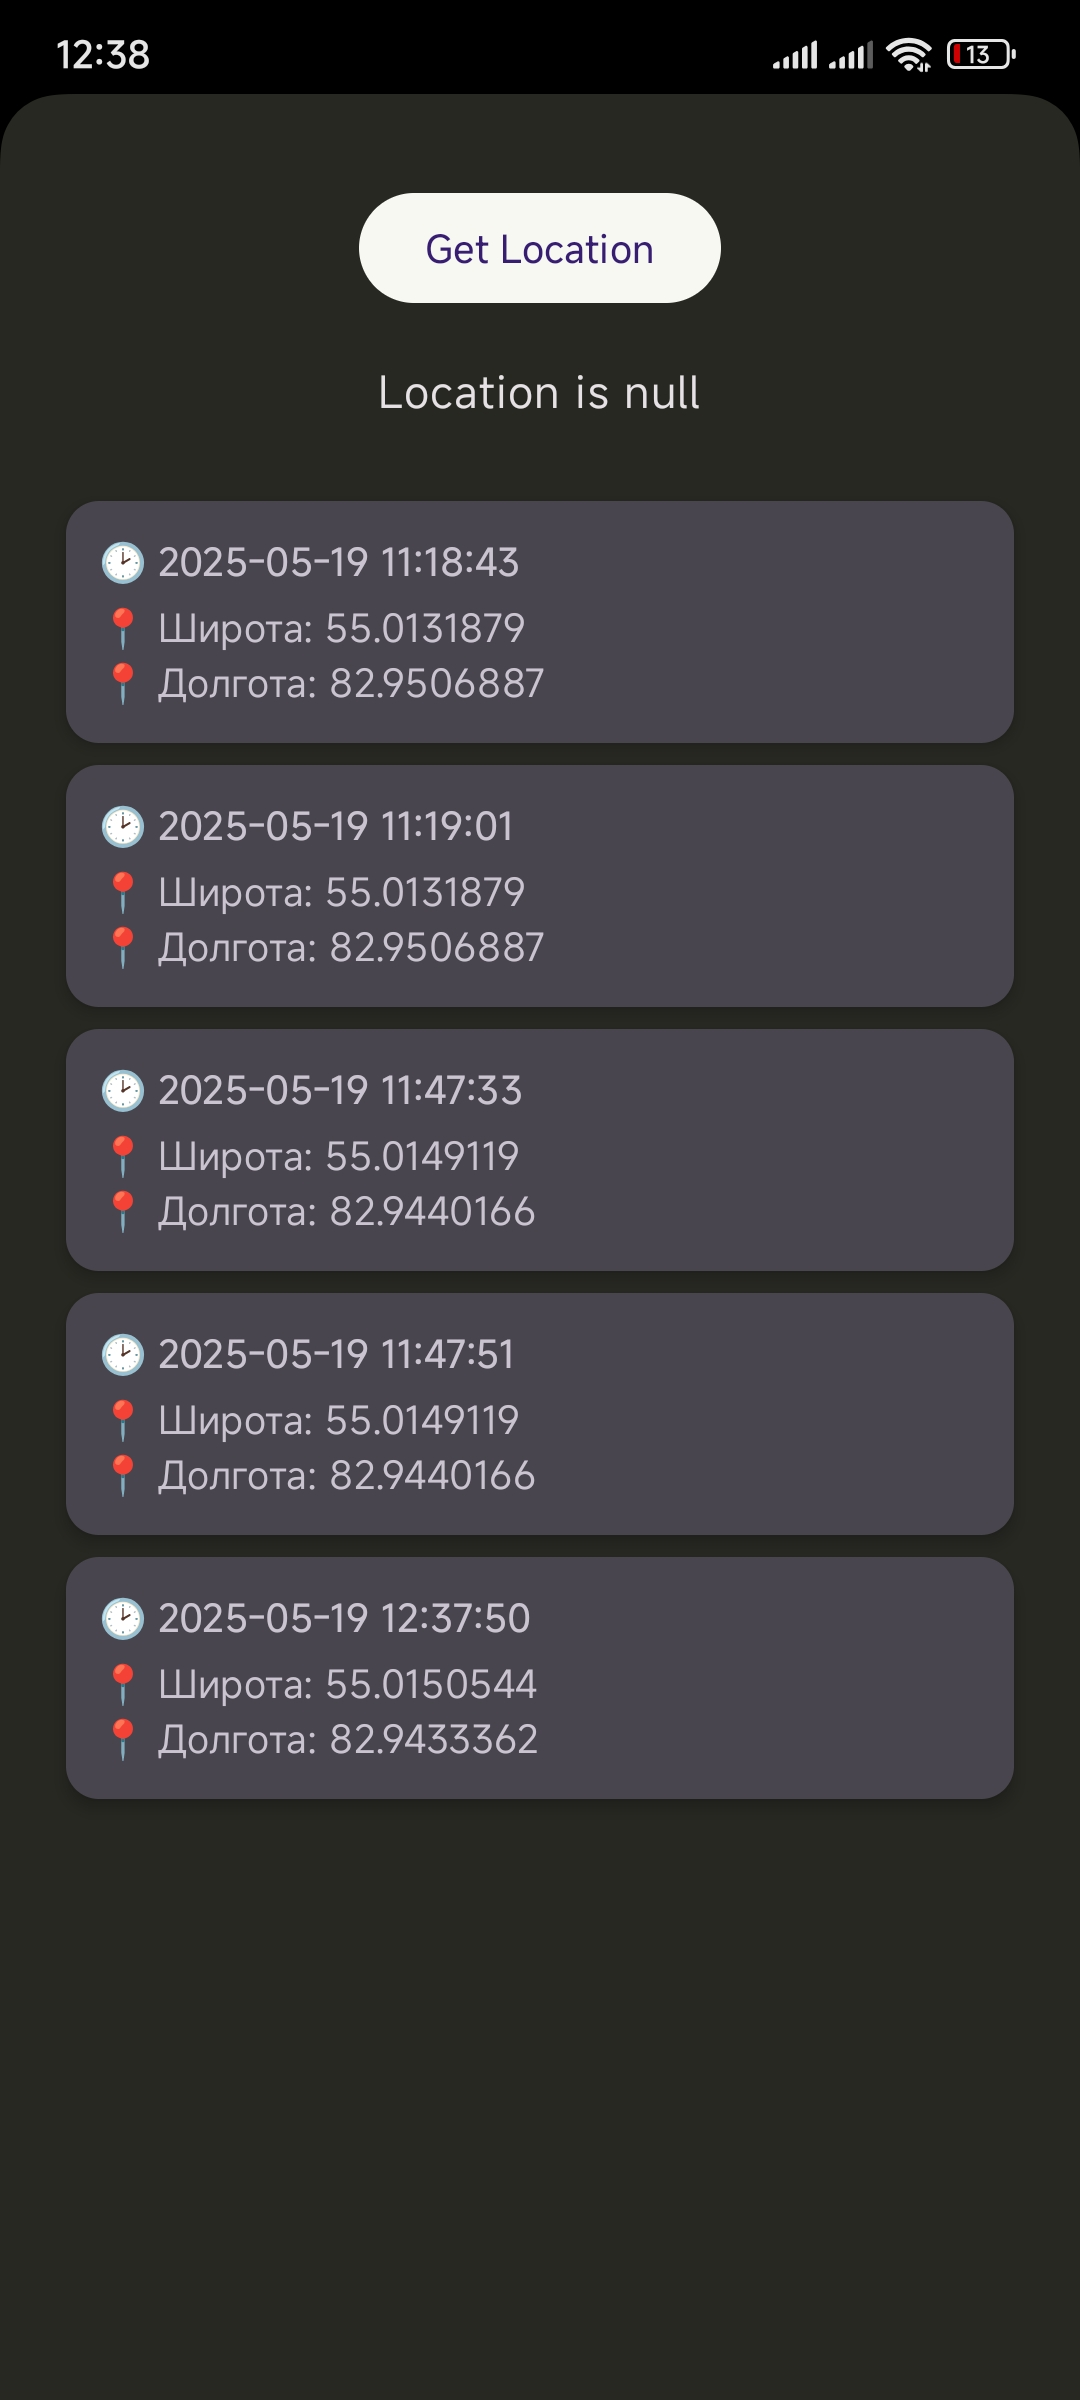
\includegraphics[width=0.5\textwidth]{is null.jpg} % путь и размер
    \caption{Location in null}
    \label{fig:myimage1}
\end{figure}

\begin{figure}[h] % h – размещение "здесь"
    \centering
    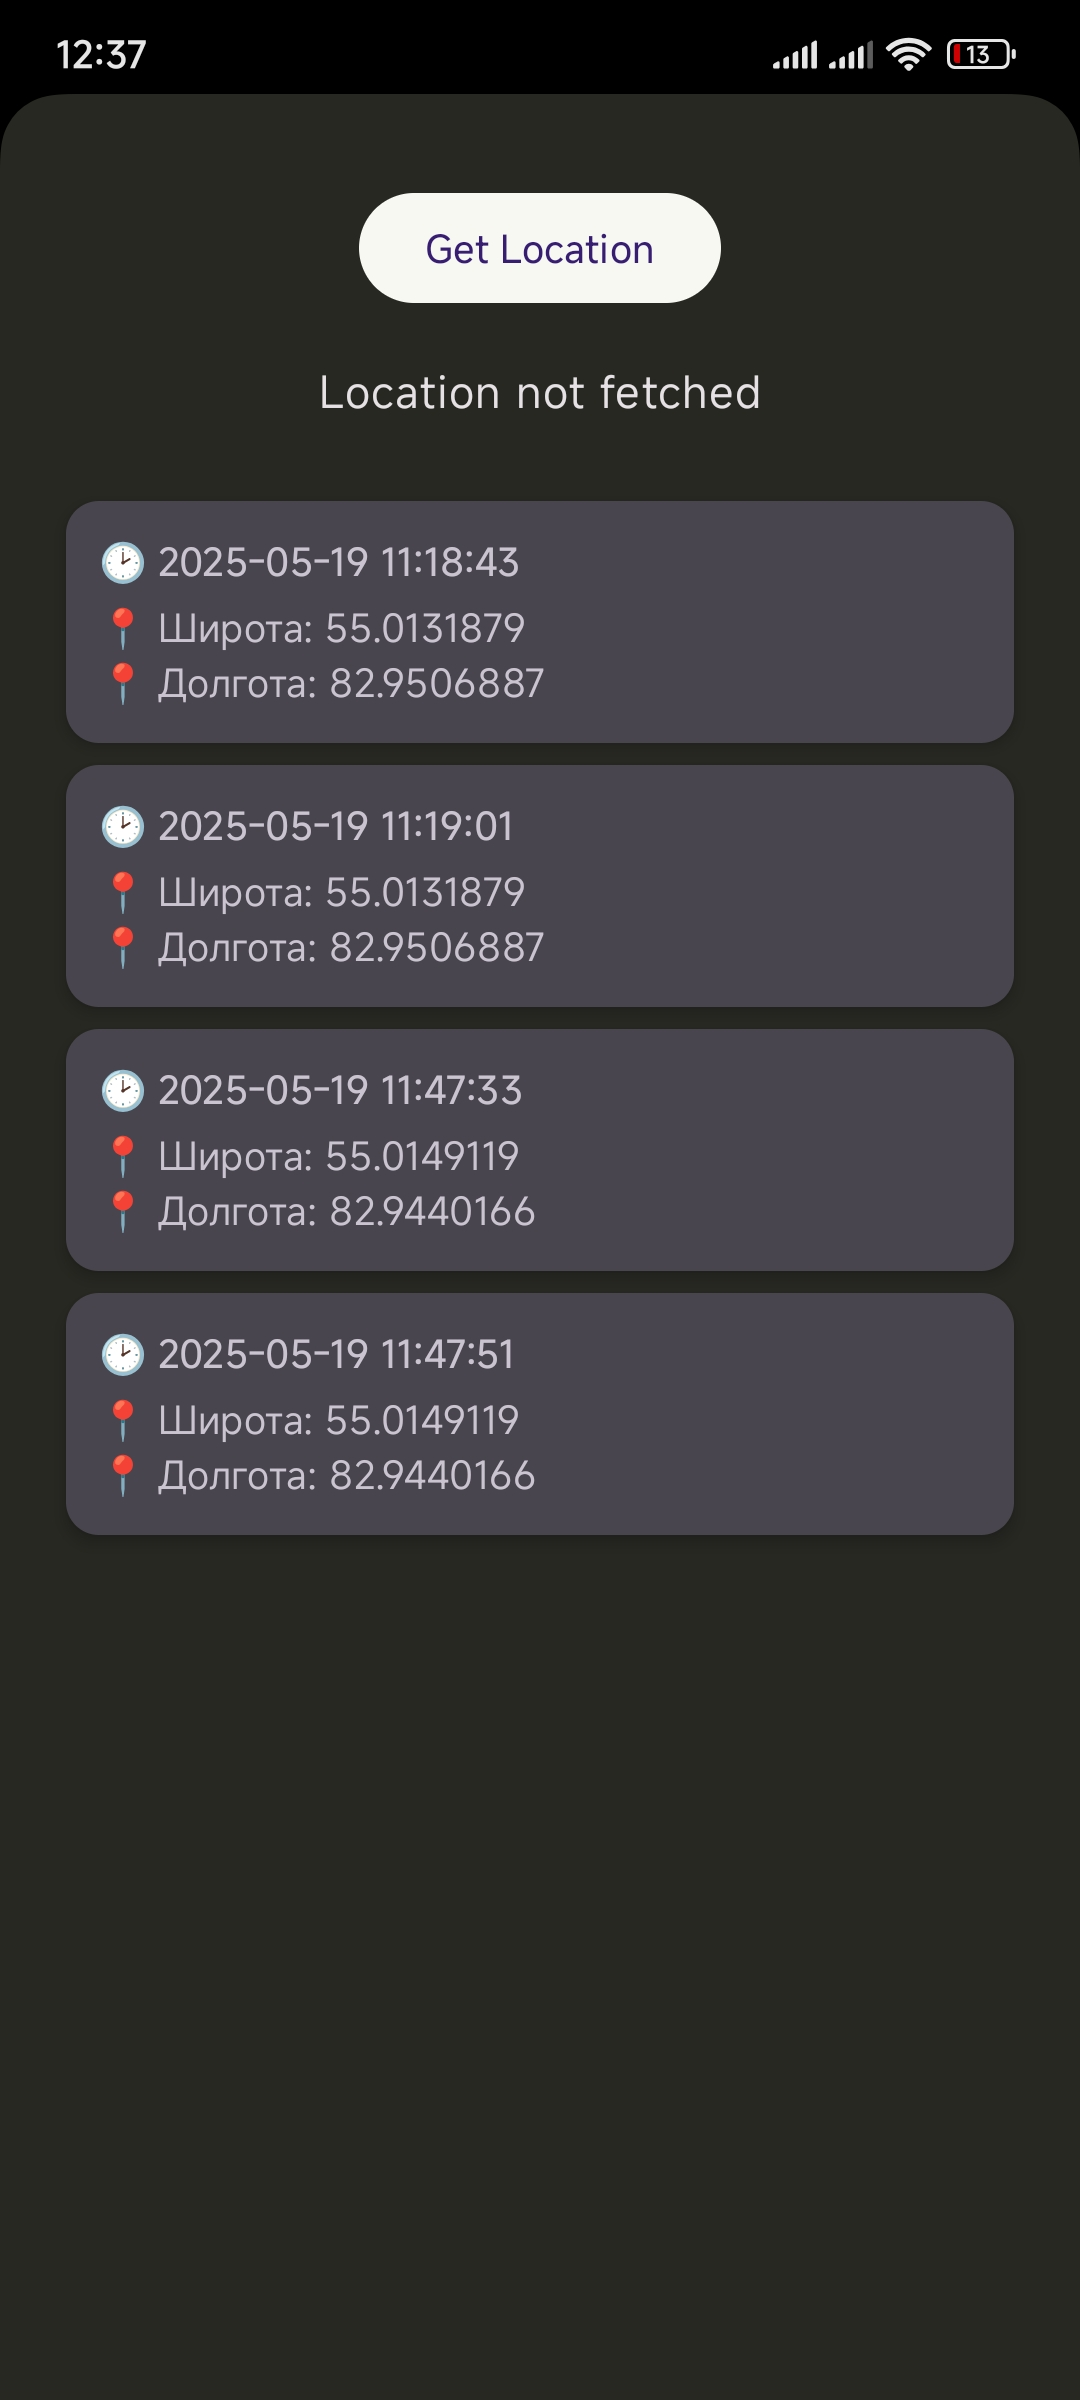
\includegraphics[width=0.5\textwidth]{not_f.jpg} % путь и размер
    \caption{Location not fetched}
    \label{fig:myimage2}
\end{figure}


\begin{figure}[h] % h – размещение "здесь"
    \centering
    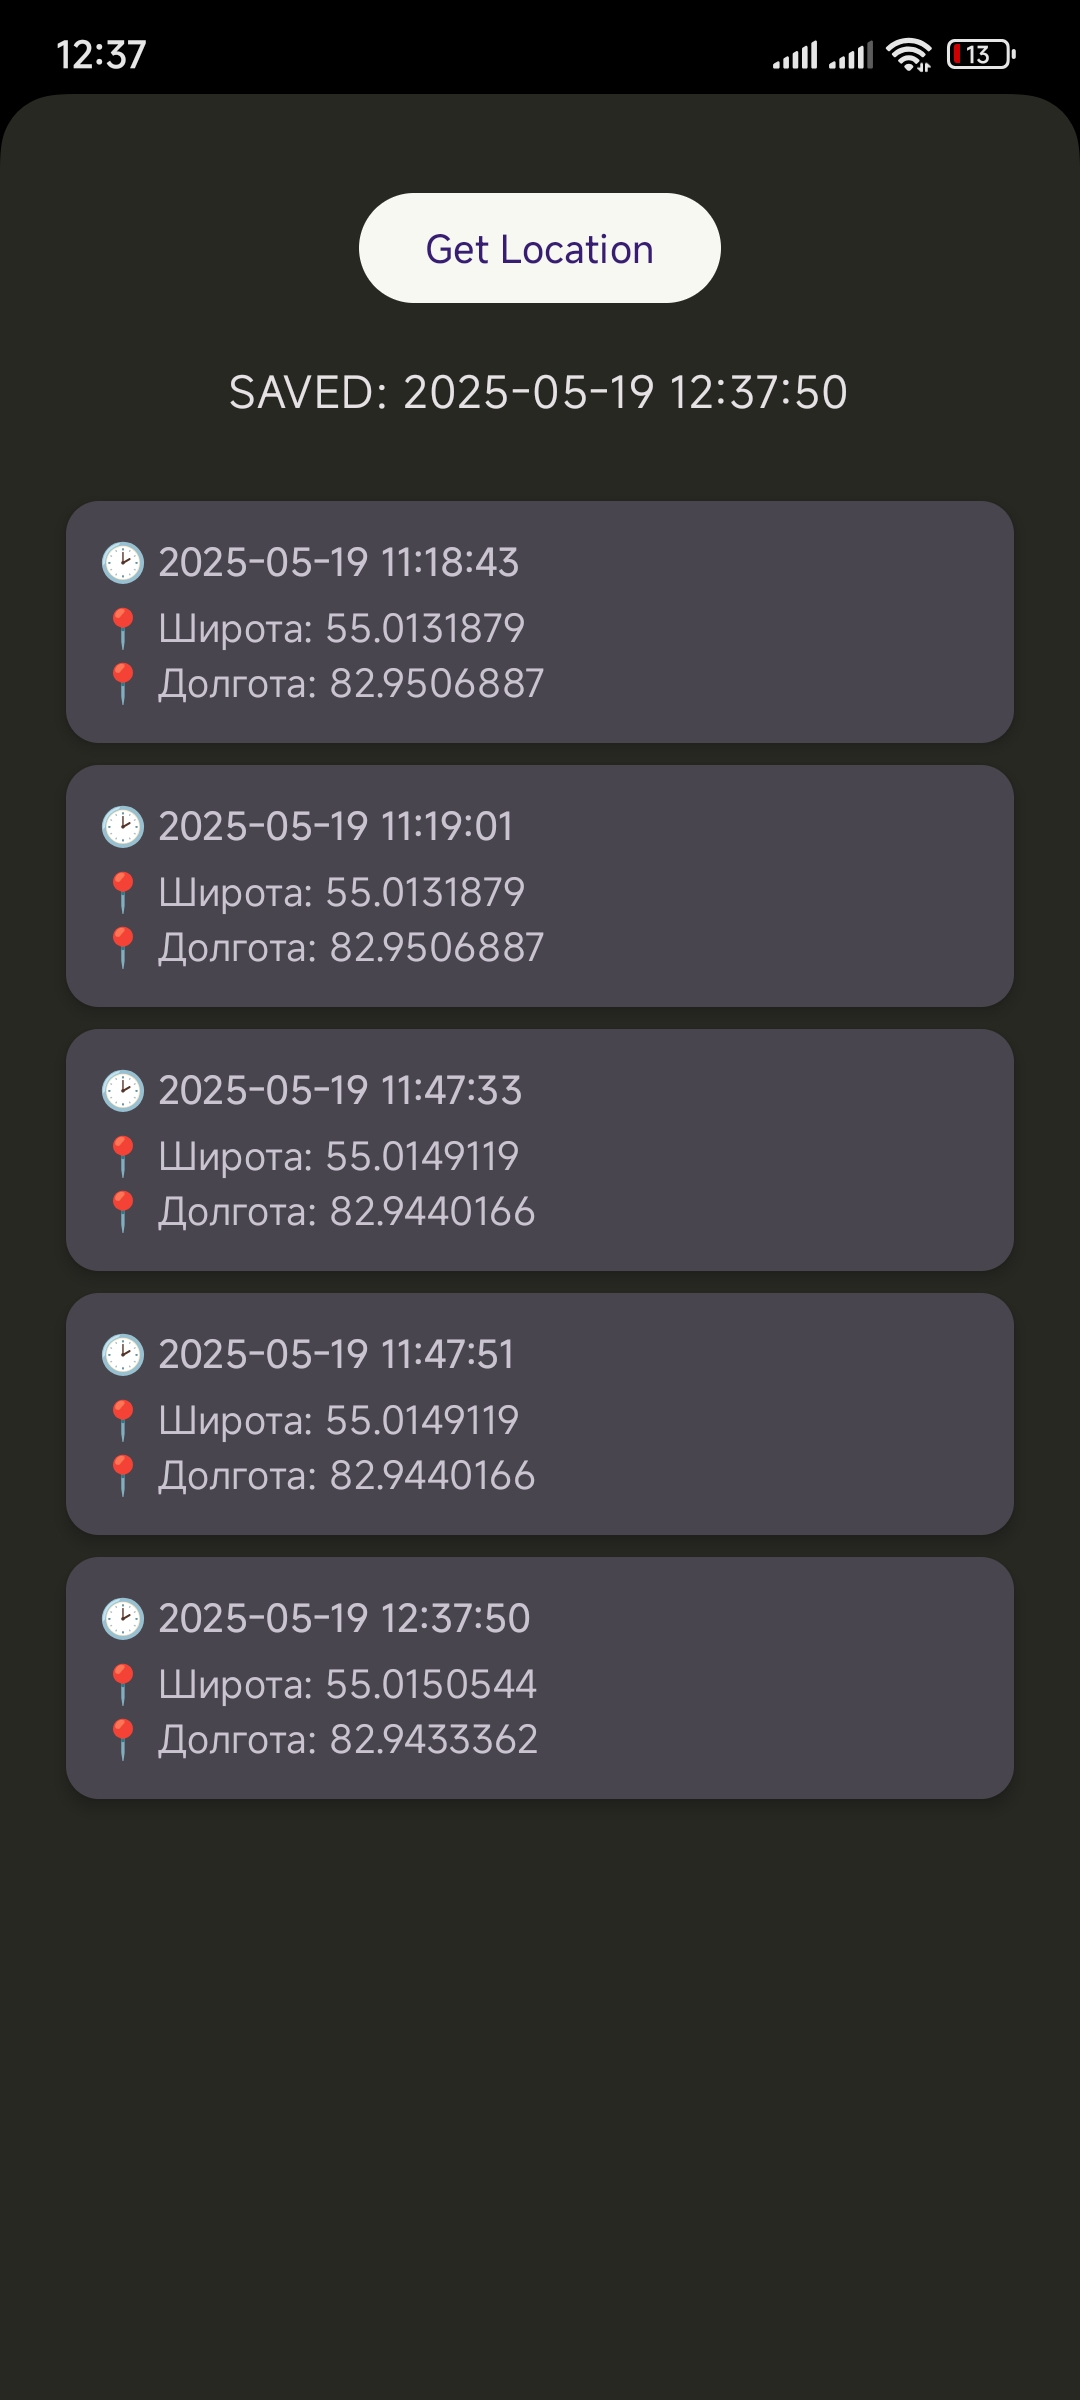
\includegraphics[width=0.5\textwidth]{saved.jpg} % путь и размер
    \caption{Location Saved}
    \label{fig:myimage3}
\end{figure}


\printbibliography[title=Список использованных источников] % Автособираемый список литературы

\end{document}